\chapter{Análisis de la situación}\label{cp: situationalAnalysis}
El estudio de la eliminación de ruido en audios o conversaciones es un problema que se empezó a estudiar muchos años atrás. Desde la aparición de la era digital el análisis y procesado de audio ha crecido mucho. Hoy en día cuando un cantante graba en estudio un disco, éstos audios se procesan digitalmente para ecualizarlos, filtrarlos o añadir efectos en el mundo digital.

Existen numerosos programas de edición y análisis de audio, desde \textit{Adobe Audition} del toolset de Adobe hasta \textit{Audacity} un programa gratuito y open-source o, incluso, Matlab\superscript{\textregistered} o Python para entornos de desarrollo o experimentación.

El procesado de audio en la actualidad consiste en, como cualquier otro análisis de señal digital, muestrear la señal, aplicarle algoritmos matemáticos a las muestras obtenidas y pasar al mundo analógico de nuevo la señal para así reproducirla en unos altavoces.

\section{Del mundo analógico al digital y viceversa}
Las señales en el mundo \textbf{analógico} son \textbf{continuas en tiempo y en valor} i.e., que para cada instante de tiempo hay un valor concreto y defino para la señal. Por el contrario una \textbf{señal digital} es \textbf{discreta en tiempo y valor} i.e., que sólo hay valores para determinados instantes de tiempo y además esos valores se encuentran determinados por el rango dinámico y la precisión del proceso de digitalización.

En primer lugar, lo que hace falta para digitalizar una señal es un sensor que transforme una magnitud física continua en una magnitud eléctrica, i.e., tensión, intensidad o resistencia. Hay infinidad de sensores que se encargan de esto en función de la magnitud física que se quiera medir. Un ejemplo sería medir temperatura con un termistor que es una resistencia variable en función de la temperatura. El sensor establece una relación entre la magnitud física objetivo y la magnitud eléctrica, de este modo, digitalizando la eléctrica se digitaliza la magnitud objetivo.

El proceso de digitalización de una señal analógica se divide en tres fases. Muestreo, cuantización y codificación. En la figura \ref{fig: adc_steps} se muestran las fases de la conversión de una señal analógica $x_a(t)$ a una señal continua en valores y discreta en tiempo $x(n)$, una señal discreta en valores y tiempo $x_q(n)$ y una señal digital representada por la salida binaria. A continuación se estudiarán brevemente el muestro y la cuantización dado el alto efecto que tienen sobre el procesamiento digital de señales. La codificación está relacionado con cómo se almacenan los bits y no es objeto de este trabajo, por ello, no se explica aquí.

\begin{figure}[ht!]
	\centering
	\resizebox{\textwidth}{!}{
			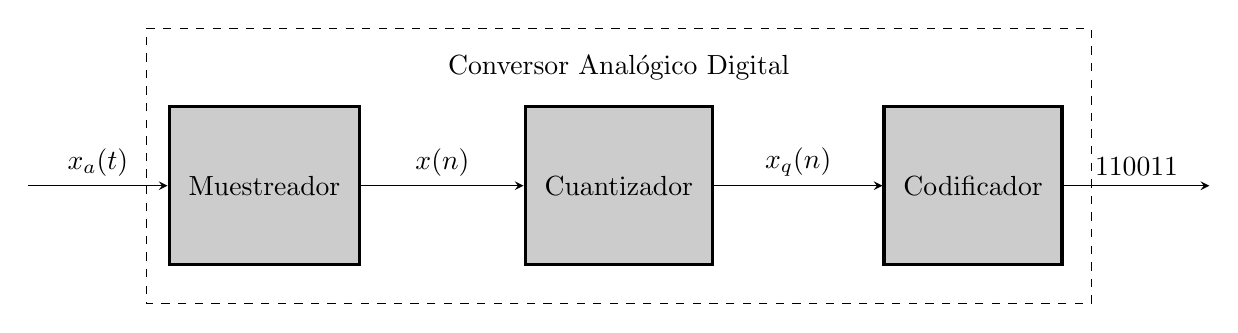
\begin{tikzpicture}
			\tikzstyle{box} = [draw,inner sep=7,minimum size=57,line 
			width=1, very thick, draw=black, fill=black!20]
			\tikzstyle{invisible} = [outer sep=0,inner sep=0,minimum size=0]
			\tikzstyle{stealth} = [-stealth]
			\node [box] (v1) at (-1,0.5) {Muestreador};
			\node [box] (v2) at (3.5,0.5) {Cuantizador};
			\node [box] (v3) at (8,0.5) {Codificador};
			\draw [stealth] (v1) edge node [anchor=south] {$x(n)$} (v2);
			\draw [stealth] (v2) edge node [anchor=south] {$x_q(n)$} (v3);
			\node [invisible] (v4) at (-4,0.5) {};
			\draw [stealth] (v4) edge node [anchor=south] {$x_a(t)$} (v1);
			\node [invisible] (v5) at (11,0.5) {};
			\draw [stealth] (v3) edge node [anchor=south] {$110011$} (v5);
			\draw [dashed] (-2.5,2.5) node [invisible] (v6) {} -- (9.5,2.5) node [invisible] {} -- 
			(9.5,-1) node [invisible] {} -- (-2.5,-1) node [invisible] {} -- (v6);
			\node [invisible] at (3.5,2) {Conversor Analógico Digital};
			\end{tikzpicture}
		}      
	\caption{Esquema de la conversión analógico a digital}
	\label{fig: adc_steps}
\end{figure}

\subsection{Muestreo}
Este proceso consiste en obtener una señal discreta en tiempo a partir de una señal continua en tiempo. Se rige por el parámetro llamado \textbf{Tasa de muestreo [sampling rate]}. Este parámetro mide el número de muestras que se van a tomar por unidad de tiempo. Es decir, define la discretización en tiempo. A mayor tasa de muestreo la señal digital podrá reproducir los cambios más rápidos de la señal. En otras palabras, podrá captar frecuencias más altas en la señal analógica. Este punto se verá con mayor detalle en \hyperref[subsec: nyquist]{\textbf{Teorema de muestreo de Nyquist-Shannon}} dado que es fundamental en el análisis de audio.

\begin{figure}[ht!]
	\centering
	\resizebox{!}{!}{
		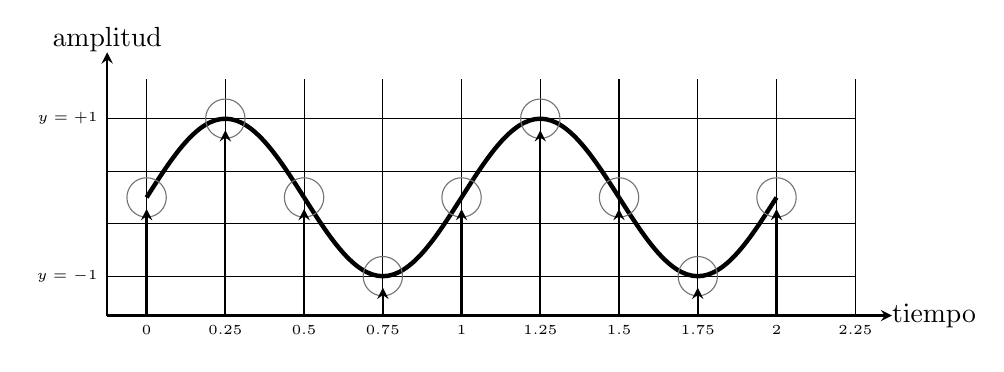
\begin{tikzpicture}
		\tikzstyle{stealth} = [-stealth, thick]
		\tikzstyle{invisible} = [outer sep=0,inner sep=0,minimum size=0]
		\tikzstyle{circle} = [shape=circle, minimum size=0.5cm, draw=black!55]
		\draw (-0.5,1)node[left,font=\tiny] {$y=+1$} -- (9,1);
		\draw (-0.5,-1)node[left,font=\tiny] {$y=-1$} -- (9,-1);
		\draw (-0.5,-0.33)node[left,font=\tiny] {} -- (9,-0.33); 
		\draw (-0.5,0.33)node[left,font=\tiny] {} -- (9,0.33); 
		\foreach \x in {0,0.25,...,2.25}
		{
			\draw (\x*4,-1.5)node [below,font=\tiny,] {\x } -- (\x*4,1.5) ;
		}
		\draw[ultra thick, ] (0,0) node (v5) {} sin (1,1) node (v7) {};
		\draw[ultra thick, ] (1,1) cos (2,0) node (v9) {};
		\draw[ultra thick, ] (2,0) sin (3,-1) node (v11) {};
		\draw[ultra thick, ] (3,-1) cos (4,0) node (v13) {};
		\draw[ultra thick, ] (4,0)  sin (5,1) node (v15) {};
		\draw[ultra thick, ] (5,1) cos (6,0) node (v17) {};
		\draw[ultra thick, ] (6,0) sin (7,-1) node (v19) {};
		\draw[ultra thick, ] (7,-1) cos (8,0) node (v21) {}; 
		\node [invisible] (v1) at (-0.5,-1.5) {};
		\node [invisible] (v2) at (-0.5,2) {amplitud};
		\node [invisible] (v3) at (10,-1.5) {tiempo};
		\draw [stealth] (v1) edge (v2);
		\draw [stealth] (v1) edge (v3);
		\node [circle] at (0,0) {};
		\node [circle] at (1,1) {};
		\node [circle] at (2,0) {};
		\node [circle] at (3,-1) {};
		\node [circle] at (4,0) {};
		\node [circle] at (5,1) {};
		\node [circle] at (6,0) {};
		\node [circle] at (7,-1) {};
		\node [circle] at (8,0) {};
		\node [invisible] (v4) at (0,-1.5) {};
		\node [invisible] (v6) at (1,-1.5) {};
		\node [invisible] (v8) at (2,-1.5) {};
		\node [invisible] (v10) at (3,-1.5) {};
		\node [invisible] (v12) at (4,-1.5) {};
		\node [invisible] (v14) at (5,-1.5) {};
		\node [invisible] (v16) at (6,-1.5) {};
		\node [invisible] (v18) at (7,-1.5) {};
		\node [invisible] (v20) at (8,-1.5) {};
		\draw [stealth] (v4) edge (v5);
		\draw [stealth] (v6) edge (v7);
		\draw [stealth] (v8) edge (v9);
		\draw [stealth] (v10) edge (v11);
		\draw [stealth] (v12) edge (v13);
		\draw [stealth] (v14) edge (v15);
		\draw [stealth] (v16) edge (v17);
		\draw [stealth] (v18) edge (v19);
		\draw [stealth] (v20) edge (v21);
		\end{tikzpicture}
	}      
	\caption{Esquema del muestreo de una señal de 1Hz muestreada a 4 muestras por segundo}
	\label{fig: sample}
\end{figure}

\subsubsection{Teorema de muestreo de Nyquist-Shannon}\label{subsec: nyquist}
Si la frecuencia más alta contenida en una señal analógica $x_{a}(t)$ es $F_{max}=B$ y la señal se muestrea a una tasa $F_{s}>2F_{max}\equiv 2B$, entonces $x_{a}(t)$ se puede recuperar totalmente a partir de sus muestras mediante la siguiente función de interpolación
\begin{align}
	g(t)&=\frac{\sin 2\pi Bt}{2\pi Bt} \\ \nonumber
	&\text{Así, }x_{a}(t)\text{ se puede expresar como:} \\ \nonumber
	x_{a}(t)&=\sum _{n=-\infty }^{\infty }x_{a}\left({\frac {n}{F_{s}}}\right)g\left(t-{\frac {n}{F_{s}}}\right)\\ \nonumber
	&\text{donde }x_{a}\left({\frac {n}{F_{s}}}\right)=x_{a}\left(nT\right)\equiv x\left(n\right)\text{ son las muestras de }x_{a}\left(t\right)
\end{align}
Esto es, que para poder recuperar una señal sin pérdida de información, ésta debe ser muestreada, al menos, con el doble de la frecuencia máxima que la señal contenga. Si no se cumpliera esto, aparecería el fenómeno del \textit{aliasing} que consiste en la superposición de componentes frecuenciales debido a un submuestreo.
\begin{figure*}[t!]
	\centering
	\begin{subfigure}[t]{0.5\textwidth}
		\centering
		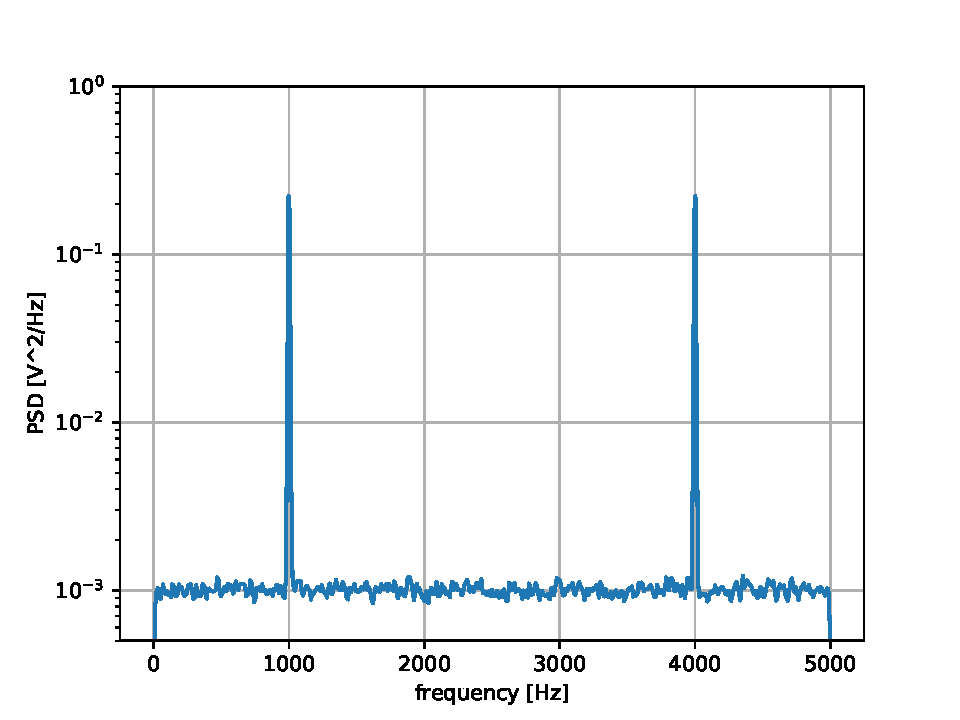
\includegraphics[width=0.9\textwidth]{figures/pwelch_1k_4k_10k}
		\caption{Densidad espectral de potencia para la suma dos senos de 1kHz y 4kHz muestreados a 10ksps}
	\end{subfigure}%
	\hspace*{10pt}
	\begin{subfigure}[t]{0.5\textwidth}
		\centering
		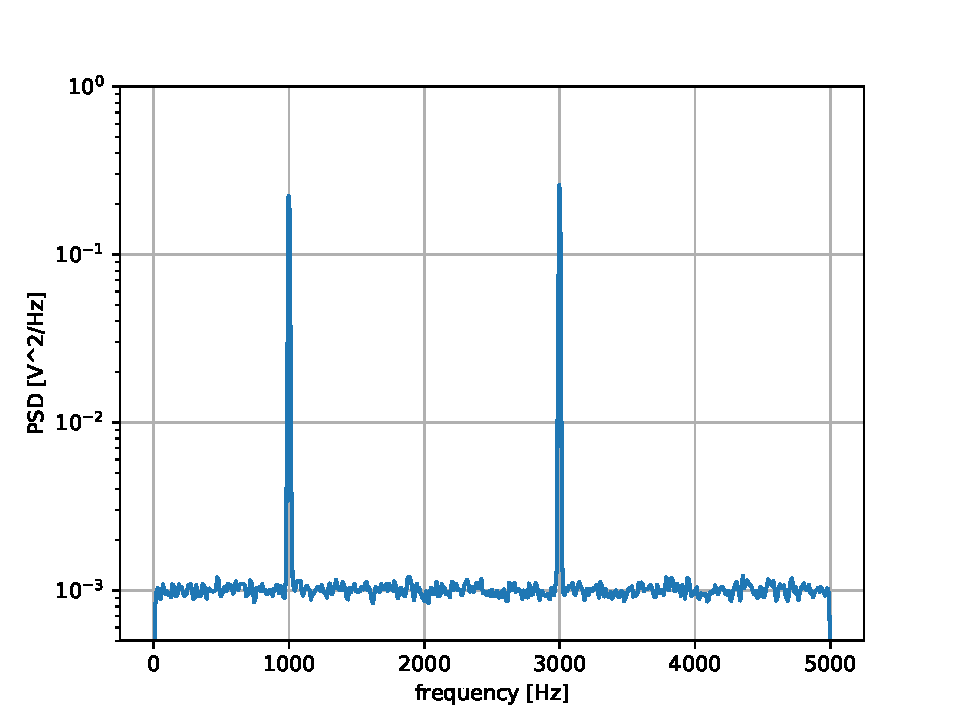
\includegraphics[width=0.9\textwidth]{figures/pwelch_1k_7k_10k}
		\caption{Densidad espectral de potencia para la suma dos senos de 1kHz y 7kHz submuestreados a 10ksps}
	\end{subfigure}
	\caption{Ejemplo de aliasing}
	\label{fig: aliasing}
\end{figure*}

En la figura \ref{fig: aliasing} se puede ver el efecto de la superposición debida al aliasing. En la primera imagen se pueden ver dos tonos a 1kHz y 4kHz respectivamente, muestreados a 10kHz. En cambio, en la segunda se ven dos tonos a 1kHz y 7kHz muestreados a 10kHz. El tono de mayor frecuencia está submuestreado por tanto los 7kHz se pliegan respecto de un eje en 5kHz apareciendo en 3kHz. De haber habido información en 3kHz ésta se hubiera superpuesto destruyendo lo que en dicha frecuencia hubiera. En la figura \ref{fig: aliasing_mirror} se muestra un esquema de lo que acaba de ocurrir, donde $\frac{f_s}{2}$ representa la mitad de la frecuencia de muestreo.

Si, la información que se encontrara más allá de la frecuencia de muestreo no fuera de interés pero no se quisiera perjudicar el ancho de banda real de la señal se debe filtrar con corte en $\frac{f_s}{2}$ para que al plegarse, el nivel de potencia sea despreciable.

\begin{figure}[ht!]
	\centering
	\resizebox{!}{!}{
		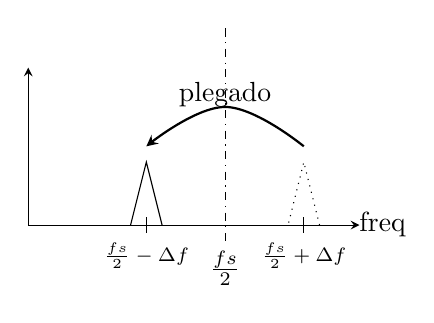
\begin{tikzpicture}
		\tikzstyle{invisible} = [outer sep=0,inner sep=0,minimum size=0]
		\tikzstyle{stealth} = [-stealth]
		\node [invisible] (v1) at (0,0) {};
		\node [invisible] (v2) at (0,2) {};
		\node [invisible] (v3) at (4.5,0) {freq};
		\draw [stealth] (v1) edge (v2);
		\draw [stealth] (v1) edge (v3);
		\draw [dashdotted](2.5,2.5) -- (2.5,-0.2) node[anchor=north]{$\frac{fs}{2}$};
		
		\draw [invisible, dotted](3.7,0) node [circle] {} -- 
		(3.5,0.8) node [circle] {} -- 
		(3.3,0) node [circle] {};
		\draw [draw](3.5,0.1) -- (3.5,-0.1) node[anchor=north]{\scriptsize$\frac{fs}{2} + \Delta f$};
		\draw [invisible](1.7,0) node [circle] {} -- 
		(1.5,0.8) node [circle] {} -- 
		(1.3,0) node [circle] {};
		\draw [draw](1.5,0.1) -- (1.5,-0.1) node[anchor=north]{\scriptsize$\frac{fs}{2} - \Delta f$};
		\draw [invisible, thick, stealth] plot[smooth, tension=.7] coordinates {(3.5,1) (2.5,1.5) (1.5,1)};
		\node [invisible, anchor=south] at (2.5,1.5) {plegado};
		\end{tikzpicture}
	}      
	\caption{Esquema del plegado de una señal con aliasing}
	\label{fig: aliasing_mirror}
\end{figure}

\subsection{Cuantización}
La cuantización consiste en obtener una señal discreta en amplitud y tiempo a partir de una señal continua en amplitud y discreta en el tiempo. Para ello, los valores de cada instante de tiempo se aproximan a los valores discretos definidos por los parámetros de la cuantización. Estos parámetros son:
\begin{itemize}
	\item \textbf{Rango dinámico [dynamic range]}. Este parámetro mide los valores máximos y mínimos hasta los cuales la señal se cuantiza. Es decir, marca los umbrales de la señal. Si los valores de la señal exceden estos límites, la señal se corta apareciendo el llamado efecto \textit{clipping}. A mayor rango dinámico para el mismo número de bits mayor rango de valores podrá obtener la señal pero con menor precisión; i.e., los saltos entre estos serán mayores.
	\item \textbf{Precisión en bits de la digitalización [\gls{ADC} number of bits]}. Este valor representa el número de escalones en los cuales se divide la escalera de cuantización. Es decir, el número de los posibles valores que puede tomar la señal digital. A mayor número de bits para el mismo rango dinámico, la precisión de la cuantización será mejor.
\end{itemize}

\begin{figure}[ht!]
	\centering
	\resizebox{!}{!}{
		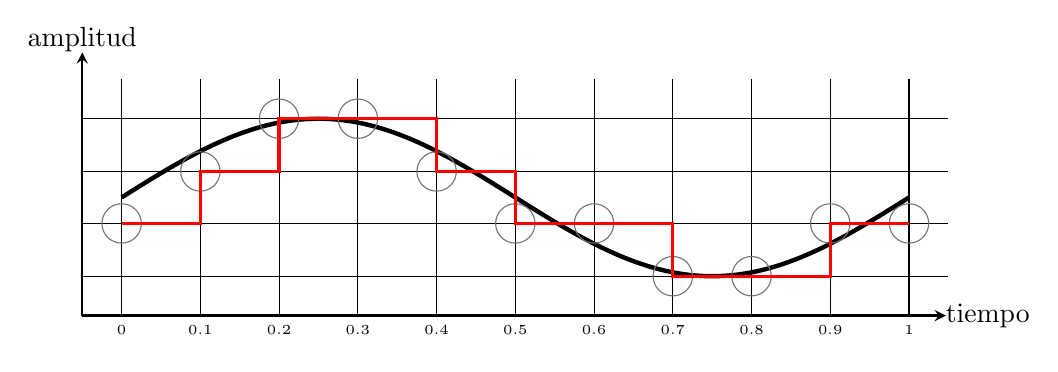
\begin{tikzpicture}
		\tikzstyle{stealth} = [-stealth, thick]
		\tikzstyle{invisible} = [outer sep=0,inner sep=0,minimum size=0]
		\tikzstyle{circle} = [shape=circle, minimum size=0.5cm, draw=black!55]
		\tikzstyle{line} = [draw, very thick, red]
		\draw (-0.5,1)node[left,font=\tiny] {} -- (10.5,1);
		\draw (-0.5,-1)node[left,font=\tiny] {} -- (10.5,-1);
		\draw (-0.5,-0.33)node[left,font=\tiny] {} -- (10.5,-0.33); 
		\draw (-0.5,0.33)node[left,font=\tiny] {} -- (10.5,0.33); 
		\foreach \x in {0,0.1,0.2,0.3,0.4,0.5,0.6,0.7,0.8,0.9,1}
		{
			\draw (\x*10,-1.5)node [below,font=\tiny,] {\x } -- (\x*10,1.5) ;
		}
		\draw[ultra thick, ] (0,0) node (v5) {} sin (2.5,1) node (v7) {};
		\draw[ultra thick, ] (2.5,1) cos (5,0) node (v9) {};
		\draw[ultra thick, ] (5,0) sin (7.5,-1) node (v11) {};
		\draw[ultra thick, ] (7.5,-1) cos (10,0) node (v13) {};
		
		\node [invisible] (v1) at (-0.5,-1.5) {};
		\node [invisible] (v2) at (-0.5,2) {amplitud};
		\node [invisible] (v3) at (11,-1.5) {tiempo};
		\draw [stealth] (v1) edge (v2);
		\draw [stealth] (v1) edge (v3);
		\node [circle] (v4) at (0,-0.33) {};
		\node [circle] (v6) at (1,0.33) {};
		\node [circle] (v8) at (2,1) {};
		\node [circle] (v10) at (3,1) {};
		\node [circle] (v12) at (4,0.33) {};
		\node [circle] (v14) at (5,-0.33) {};
		\node [circle] at (6,-0.33) {};
		\node [circle] (v15) at (7,-1) {};
		\node [circle] at (8,-1) {};
		\node [circle] (v16) at (9,-0.33) {};
		\node [circle] (v17) at (10,-0.33) {};
		\draw [line](0,-0.33) -- (1,-0.33) node [invisible] {} -- (1,0.33) -- 
		(2,0.33) node [invisible] {} -- (2,1) -- 
		(4,1) node [invisible] {} -- (4,0.33) -- 
		(5,0.33) node [invisible] {} -- (5,-0.33) -- 
		(7,-0.33) node [invisible] {} -- (7,-1) -- 
		(9,-1) node [invisible] {} -- (9,-0.33) -- (10,-0.33);
		\end{tikzpicture}
	}      
	\caption{Esquema de la cuantización con 2 bits a 10 muestras por segundo, i.e., 4 valores posibles}
	\label{fig: cuantization_2bit}
\end{figure}

\begin{figure}[ht!]
	\centering
	\resizebox{!}{!}{
		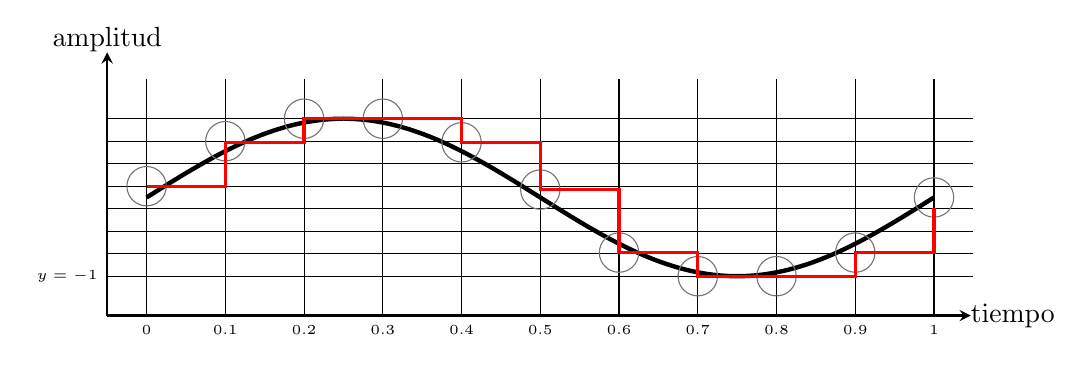
\begin{tikzpicture}
		\tikzstyle{stealth} = [-stealth, thick]
		\tikzstyle{invisible} = [outer sep=0,inner sep=0,minimum size=0]
		\tikzstyle{circle} = [shape=circle, minimum size=0.5cm, draw=black!55]
		\tikzstyle{line} = [draw, very thick, red]
		\draw (-0.5,1)node[left,font=\tiny] {} -- (10.5,1);
		\draw (-0.5,0.7142)node[left,font=\tiny] {} -- (10.5,0.7142);
		\draw (-0.5,0.4285)node[left,font=\tiny] {} -- (10.5,0.4285);
		\draw (-0.5,0.1428)node[left,font=\tiny] {} -- (10.5,0.1428);
		\draw (-0.5,-0.1428)node[left,font=\tiny] {} -- (10.5,-0.1428);
		\draw (-0.5,-0.4285)node[left,font=\tiny] {} -- (10.5,-0.4285);
		\draw (-0.5,-0.7142)node[left,font=\tiny] {} -- (10.5,-0.7142);
		\draw (-0.5,-1)node[left,font=\tiny] {$y=-1$} -- (10.5,-1);
		\foreach \x in {0,0.1,0.2,0.3,0.4,0.5,0.6,0.7,0.8,0.9,1}
		{
			\draw (\x*10,-1.5)node [below,font=\tiny,] {\x } -- (\x*10,1.5) ;
		}
		\draw[ultra thick, ] (0,0) node (v5) {} sin (2.5,1) node (v7) {};
		\draw[ultra thick, ] (2.5,1) cos (5,0) node (v9) {};
		\draw[ultra thick, ] (5,0) sin (7.5,-1) node (v11) {};
		\draw[ultra thick, ] (7.5,-1) cos (10,0) node (v13) {};
		
		\node [invisible] (v1) at (-0.5,-1.5) {};
		\node [invisible] (v2) at (-0.5,2) {amplitud};
		\node [invisible] (v3) at (11,-1.5) {tiempo};
		\draw [stealth] (v1) edge (v2);
		\draw [stealth] (v1) edge (v3);
		\node [circle] (v4) at (0,0.1428) {};
		\node [circle] (v6) at (1,0.7142) {};
		\node [circle] (v8) at (2,1) {};
		\node [circle] (v10) at (3,1) {};
		\node [circle] (v12) at (4,0.7) {};
		\node [circle] (v14) at (5,0.1) {};
		\node [circle] at (6,-0.7) {};
		\node [circle] (v15) at (7,-1) {};
		\node [circle] at (8,-1) {};
		\node [circle] (v16) at (9,-0.7) {};
		\node [circle] (v17) at (10,0) {};
		\draw [line](0,0.1428) -- (1,0.1428) node [invisible] {} -- (1,0.7) -- 
		(2,0.7) node [invisible] {} -- (2,1) -- 
		(4,1) node [invisible] {} -- (4,0.7) -- 
		(5,0.7) node [invisible] {} -- (5,0.1) node [invisible] {} --
		(6,0.1) -- (6,-0.7) node [invisible] {} --
		(7,-0.7) node [invisible] {} -- (7,-1) -- 
		(9,-1) node [invisible] {} -- (9,-0.7) -- (10,-0.7) -- (10,-0.14);
		\end{tikzpicture}
	}      
	\caption{Esquema de la cuantización con 4 bits a 10 muestras por segundo, i.e., 8 valores posibles}
	\label{fig: cuantization_4bit}
\end{figure}

En las figuras \ref{fig: cuantization_2bit} y \ref{fig: cuantization_4bit} se pueden ver ejemplos de una cuantización con 2 y 4 bits respectivamente.

\begin{figure}[ht!]
	\centering
	\resizebox{!}{!}{
		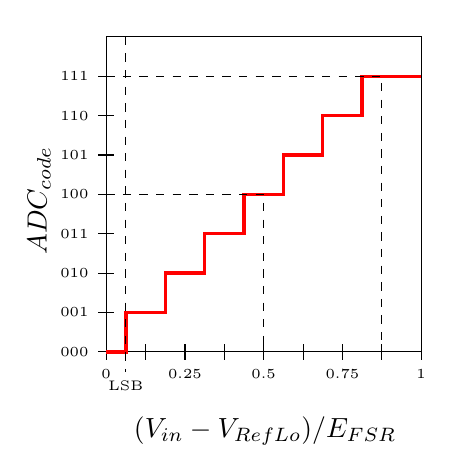
\begin{tikzpicture}
		\tikzstyle{stealth} = [-stealth, thick]
		\tikzstyle{invisible} = [outer sep=0,inner sep=0,minimum size=0]
		\tikzstyle{circle} = [shape=circle, minimum size=0.5cm, draw=black!55]
		\tikzstyle{line} = [draw, very thick, red]
		
		\draw (0,0) node [invisible] (v1) {} --
		(4,0) node [invisible] {} --
		(4,4) node [invisible] {} --
		(0,4) node [invisible] {} --
		(0,0) node [invisible] {};
		\foreach \x in {0,0.25,0.5,0.75,1}
		{
			\draw (\x*4,-0.1)node [below,font=\tiny,] {\x } -- (\x*4,0.1) ;
		}
		\foreach \x in {0.125,0.375,0.625,0.875,1}
		{
			\draw (\x*4,-0.1)node [below,font=\tiny,] {} -- (\x*4,0.1);
		}
		\foreach \c [count=\x from 0] in {{000},{001},{010},{011},{100},{101},{110},{111}}
		{
			\draw (-0.1,\x*0.5)node [anchor=east,font=\tiny,] {\c} -- (0.1,\x*0.5);
		}
		%\node at (0,\x) {\c};	
		\draw [line](v1) -- (0.25,0) node [invisible] {} -- 
		(0.25,0.5) node [invisible] {} -- 
		(0.75,0.5) node [invisible] {} -- 
		(0.75,1) node [invisible] {} -- 
		(1.25,1) node [invisible] {} -- 
		(1.25,1.5) node [invisible] {} -- 
		(1.75,1.5) node [invisible] {} -- 
		(1.75,2) node [invisible] {} -- 
		(2.25,2) node [invisible] {} -- 
		(2.25,2.5) node [invisible] {} -- 
		(2.75,2.5) node [invisible] {} -- 
		(2.75,3) node [invisible] {} -- 
		(3.25,3) node [invisible] {} -- 
		(3.25,3.5) node [invisible] {} -- 
		(4,3.5) node [invisible] {};
		\node [invisible] at (2.0187,-1) {$(V_{in}-V_{RefLo})/E_{FSR}$};
		\node [invisible, rotate=90] at (-0.8509,1.9232) {$ADC_{code}$};
		\draw [dashed](0,2) node [invisible] {} -- (2,2) node [invisible] {} -- (2,0) node [invisible] {};
		\draw [dashed](0,3.5) node [invisible] {} -- (3.5,3.5) node [invisible] {} -- (3.5,0) node [invisible] {};
		\draw [dashed](0.25,4) node [] {} -- (0.25,-0.25) node [anchor=north] {\tiny LSB};
		\end{tikzpicture}
	}      
	\caption{Resolución del \gls{ADC}}
	\label{fig: adc_resolution}
\end{figure}

En la figura \ref{fig: adc_resolution} se muestra la escalera de cuantización con la resolución del \gls{ADC} calculada como se muestra en \ref{eq: adc_resolution}
\begin{align}
Q&=\frac{E_{FSR}}{2^M}\text{ donde,} \\ \nonumber
E_{FSR}&= V_{RefHi}\text{-}V_{RefLow} \\ \nonumber
\text{siendo }&V_{RefHi}\text{ el voltaje máximo de referencia}\\ \nonumber
&V_{RefLow}\text{ el voltaje mínimo de referencia y}\\ \nonumber
&M\text{ el número de bits de precisión}
\end{align}\label{eq: adc_resolution}

\section{Proceso tradicional vs redes neuronales}
El proceso tradicional consiste en procesar la señal digital con técnicas de \gls{DSP}. Estas técnicas pueden ser de muchos tipos y aplicadas tanto en el dominio del tiempo como en el dominio de la frecuencia. Este tipo de procesado es muy efectivo pero tiene el inconveniente de que si no está lo bastante adaptado para el problema en cuestión, destruye información válida en lugar de limpiar el ruido. Este proceso de afinado \textit{fine tuning} es una tarea tediosa y no siempre aplica del mismo modo dado que pequeñas variaciones en el entorno hacen que haya que tunear de nuevo la cadena de procesado de señal.

En contrapartida, están las redes neuronales que, siendo entrenadas con un gran abanico de señales y de ruidos pueden aprender a discernir patrones para limpiar así las señales del ruido. Estos algoritmos son computacionalmente costosos en comparación al \gls{DSP} tradicional. Es por ello que algunos autores han realizado sistemas híbridos en los cuales el procesado se hace con \gls{DSP} y el tuneo fino con redes neuronales. De este modo, se obtienen buenas características de ambos, pero sigue existiendo la limitación del procesado tradicional de \gls{DSP} que se limita a la cadena de procesado programada, i.e., las etapas de procesado son estáticas en diseño o su morfología no se adapta según las variaciones del entorno.

\section{Redes neuronales para series temporales}
